%\documentstyle[epsf,twocolumn]{jarticle}       %LaTeX2.09仕様
%\documentclass[twocolumn]{jarticle}     %pLaTeX2e仕様
\documentclass{jarticle}     %pLaTeX2e仕様

%一枚組だったら[twocolumn]関係のとこ消す

\setlength{\topmargin}{-45pt}
%\setlength{\oddsidemargin}{0cm} 
\setlength{\oddsidemargin}{-7.5mm}
%\setlength{\evensidemargin}{0cm} 
\setlength{\textheight}{24.1cm}
%setlength{\textheight}{25cm} 
\setlength{\textwidth}{17.4cm}
%\setlength{\textwidth}{172mm} 
\setlength{\columnsep}{11mm}

\kanjiskip=.07zw plus.5pt minus.5pt

\usepackage{graphicx}
\usepackage[dvipdfmx]{color}
\usepackage{subcaption}
\usepackage{enumerate}
\usepackage{comment}
\usepackage{url}
\usepackage{multirow}
\usepackage{diagbox}
\usepackage{amsmath,amssymb}
\usepackage{mathtools}
\usepackage{wrapfig}
\usepackage{graphicx}
\usepackage{float}
\usepackage{algorithmic}
\usepackage{algorithm}

\begin{document}
  \noindent
  \onecolumn
  \hspace{1em}

  \today
  \hfill
  \ \  B3 西村昭賢 

  \vspace{2mm}
  \hrule
  \begin{center}
  {\Large \bf 進捗報告}
  \end{center}
  \hrule
  \vspace{3mm}


\section{今週やったこと}
\begin{itemize}
  \item 研究発表会で頂いた指摘, アドバイスについての考察
  \item ランダムに行動するプレイヤー同士の勝率計算
\end{itemize}

\section{研究発表会で頂いた質問, アドバイスについての考察}
\begin{itemize}
  \item DQN で action がどのように決まるのか
  \par
  DQN では, 図 に示した疑似コード \cite{DQN} における下から3行目で計算する loss を最小化するように学習し Q値を更新する.
  DQN の実装で用いた keras-rl では, 方策に基づいて action を決定する際に, それぞれの action (離散値) に対して Q 値の推定値を算出する \cite{keras-rl} .
  実験で用いた $\mathrm{\epsilon}$ - greedy では, 確率 $\mathrm{\epsilon}$ でランダムに行動し, それ以外では算出された Q 値の推定値から最も値が大きい action を選択する.
  \par
  このため, 質問にあったような action が 8.5 とかになって 8 と 9 のどちらかを選ぶ状況にはならない. そもそも DQN は離散的な行動空間にしか対応していない.
  \begin{figure}[h]
    \centering
    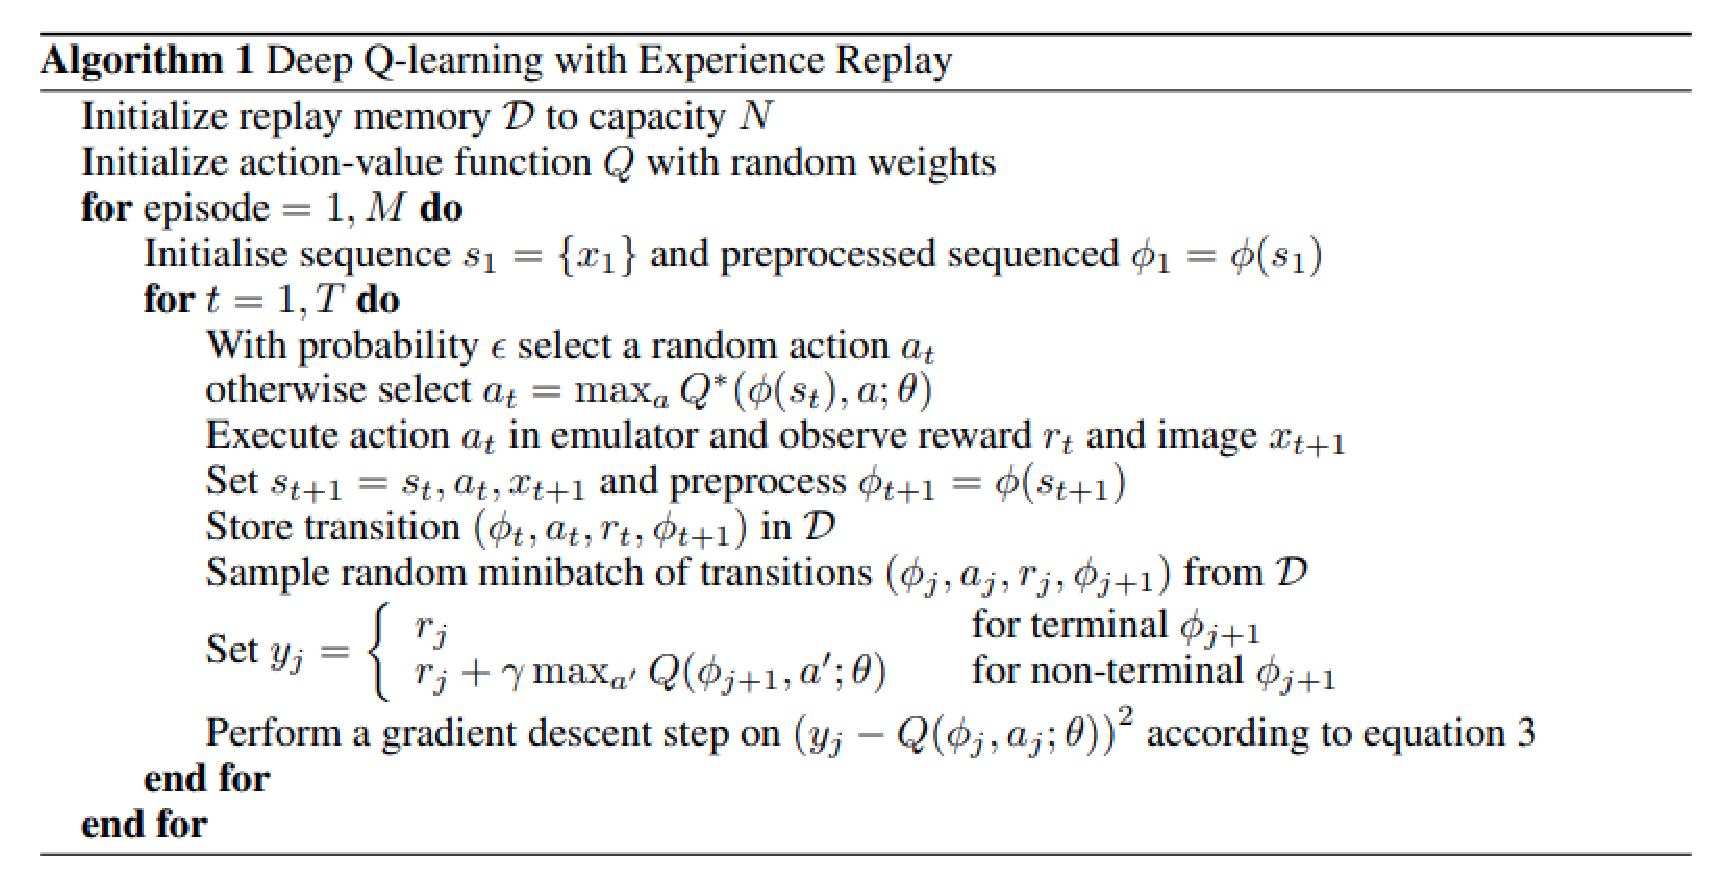
\includegraphics[width=120mm]{assets/DQNalgo.eps}
    \caption{DQN の疑似コード \cite{DQN}}
    \label{fig:result4}
  \end{figure}

  \item 標準偏差が学習進むにつれて小さくならないのか
  \par
  これも, $\mathrm{\epsilon}$ - greedy によるものと考えられる. 学習が安定してからも確率 $\mathrm{\epsilon}$ でランダムに行動するため, 平均を取るエピソード数の勝敗にばらつきが発生すると考えられる.

  \item 考察に学習プレイヤーの学習序盤と学習後期の行動の比較, 人間が考える最善手との比較を含めるべき
  \par
  資料や発表でどのように示すかが難しそうと考えた. 現在は学習済みモデルにおいて 5 エピソードくらいのログを見てどのように行動しているか判断している. 例えば先週の資料では, 「学習したエージェントの行動を見てみると先攻プレイヤーらしく, 積極的に相手プレイヤーに攻撃し, 手札からも攻撃の特殊効果を持つカードを優先的にプレイしていた.」といったように記載した. 
  \par 
  これだけだと主観的すぎると考えた. そのため勝利時に盤面にプレイした平均枚数をカードごとに算出できるようにした. これで学習プレイヤーがどのカードを重視して盤面にプレイしているかを示すことができる. 
  しかし, これだけでは盤面での行動の様子が数字として示せない. 各カードについてどのカードを攻撃したか, 相手プレイヤーに直接攻撃したか回数を測定すれば盤面のカードについての傾向が示せるのではないかと現時点では考えている. 

  \item どこに新規性があるのかはっきり言えるようにしておくべき
  \par
  森先生と相談した. 
  \par
  バランス調整という抽象的な概念について, 定量的に評価する. それを構築環境で実験することに新規性がある.

\end{itemize}


\section{ランダムに行動するプレイヤー同士の勝率計算}
バランス調整に取り組むにあたり, まずはランダムに行動するプレイヤー同士の勝利を計算できるようにした.
ランダムに行動するプレイヤーは, 表 \ref{table:action2-2} に示す行動空間に沿って, 取りうる行動の中からランダムに行動を選択して行動する.
\begin{table}[t]
  \centering
  \caption{ランダムに行動するプレイヤーの行動空間}
  \label{table:action2-2}
  \begin{tabular}{|c|c|}
  \hline
  行動説明                          & 次元数        \\ \hline
  手札 1 $\sim$ 9 を自盤面に出す             & 9          \\ \hline
  自盤面 1 が敵盤面 1 $\sim$ 5 に攻撃 or 敵プレイヤーに攻撃    & 6          \\ \hline
  自盤面 2 が敵盤面 1 $\sim$ 5 に攻撃 or 敵プレイヤーに攻撃    & 6   \\ \hline
  自盤面 3 が敵盤面 1 $\sim$ 5 に攻撃 or 敵プレイヤーに攻撃    & 6\\ \hline
  自盤面 4 が敵盤面 1 $\sim$ 5 に攻撃 or 敵プレイヤーに攻撃    & 6 \\ \hline
  自盤面 5 が敵盤面 1 $\sim$ 5 に攻撃 or 敵プレイヤーに攻撃    & 6\\ \hline
  ターンエンド & 1 \\ \hline
  \end{tabular}
  \end{table}
なお, 記載ミスで前回の資料で示した実験は全てゲーム開始時に初期手札としてカードを 5 枚ドローしていた.
手札のマリガンといった操作がないため意図的に変更していたが変更を記録していなかった. 申し訳ありません.
\par
今回ではゲーム開始時の初期手札枚数を 3 枚に戻し, ランダム同士の対戦, 先週の資料で示したアグロ的な戦略同士の対戦を 10000 回実行し先攻の勝率を計算した.表 \ref{table:result} に結果を示す.
先週, アグロ同士の先攻の勝率は 0.6425 であったが , 初期手札の枚数が減り運要素が高まったためさらに先攻有利に傾いた.

\begin{table}[t]
  \centering
  \caption{10000 回対戦し計算した先攻の勝率 (戦略はミラー)}
  \vspace{-0.3cm}
  \label{table:result}
  \scalebox{1.0}[1.0]{
    \begin{tabular}{|c|c|}
      \hline
      戦略 & 勝率 \\ \hline
      ランダム & 0.5011 \\ \hline
      アグロ & 0.6661 \\ \hline
  
      \end{tabular}
  }
  \end{table}

\section{今後やること (優先度高い順)}
\begin{itemize}
  \item 「何もしない」を行動空間に含めた際に, 「何もしない」が損であると学習しているかどうか確認
  \par
  盤面, 手札のカードに対して「何もしない」という行動を加えた行動空間で 100000 ステップほど学習させた結果, 改良した $\mathrm{\epsilon}$ - greedy が指数関数的に減少するため学習のかなり序盤で $\mathrm{\epsilon}$ が最小値を取り局所解に入ってしまい上手く学習が進まなかった.
  先週, 手札に対して「何もしない」行動を加えた行動空間では, 改良した $\mathrm{\epsilon}$ - greedy で学習できたためその行動空間に変更し確認してみる.
  \item バランス調整
  \par
  ランダム同士でほぼ五分五分の勝率であったため, 実験として後攻の勝率が 55 \% 以上になるまでパラメータを調整してみる. 調整するパラメータは, 現段階では 「後攻の初期手札の枚数」, 「後攻の HP 最大値」 , 「後攻のコスト初期値」の 3 つを考えている.
  \item 構築環境の改良
  \par
  アグロが最適解の環境になっているため, ブロッキングと全破壊の特殊効果を追加して DQN を適用して学習プレイヤーの行動を観測する.
  \item 各カードについてどのカードを攻撃したか, 相手プレイヤーに直接攻撃したか回数を測定
  \par
  DQN の適用実験の結果として必要.
\end{itemize}


%index.bibはtexファイルと同階層に置く
%ちゃんと\citeしないと表示されない(1敗)
\bibliography{index.bib}
\bibliographystyle{junsrt}

\end{document}